 \documentclass[amsmath,preprintnumbers,10pt,nofootinbib,prl,twocolumn]{revtex4-1}
\usepackage{amsbsy}
\usepackage{amsmath}
\usepackage{amssymb}
\usepackage{graphicx}
\usepackage{color}
\usepackage{subfig}
\usepackage{physics}
\usepackage{soul}
\usepackage{color}
\usepackage{bm}
\usepackage[normalem]{ulem}

%\newcommand{\Tr}{\text{Tr}}
\newcommand{\Ai}{\text{Ai}}
\newcommand{\Bi}{\text{Bi}}
\newcommand{\Real}{\text{Re}}
\newcommand{\Imag}{\text{Im}}

\usepackage{verbatim}
\usepackage{natbib}
\bibliographystyle{apsrev4-1}
\begin{document}
\title{Supplementary Information: Dissipation induced transitions in two dimensional elastic membranes.}
\author{Michael Nguyen$^{1,2}$, Suriyanarayanan Vaikuntanathan$^{1,2}$} 
\affiliation{$^1$The James Franck Institute, The University of Chicago, Chicago, IL,}
\affiliation{$^2$ Department of Chemistry, The University of Chicago, Chicago, IL.}
\maketitle
\section{Move set for adding and removing particles in the Monte-Carlo simulations}
Fig.~\ref{fig:SimulationSchematic} describes the procedure used to simulate addition and removal moves in our numerical calculations. The initial configuration of the assembly is a circle consisting of $N_0$ particles with equal distance between them. Additional and removal events are chosen with equal probability. In an additional move, first a random particle in the assembly is chosen. As described in Fig.~\ref{fig:SimulationSchematic}, an additional move is attempted in a region between the chosen random particle and the next particle in the clockwise direction. The area of the region is kept constant.  An addition move is  accepted with the probability $\rm{Min}(\rm{Exp}[-\Delta E +\mu],1)$. In a removal move,  a random particle is simply removed from the assembly with the probability $\rm{Min}(\rm{Exp}[-\Delta E -\mu],1)$. The transition rates of the simulations are:
\begin{equation}
W^{N,N+1}_{ij}=P_i(\bold{l},\bold{\theta})\frac{1}{AN}\rm{Min(Exp[-(E_j - E_i)+\mu],1)}
\end{equation}
\begin{equation}
W^{N+1,N}_{ij}=P_j(\bold{l},\bold{\theta})\frac{1}{N+1}\rm{Min(Exp[-(E_i - E_j)-\mu],1)}
\end{equation}

With the above rules, we then start the growing simulation. Each Monte-Carlo step in the simulation is an attempt to add or remove a particle. Each simulation is run for at least $10^9$ Monte-Carlo steps. After the simulation finishes, we measure the fluctuation of the particles about its center as described in the main text. For each value of $\delta\mu$, at least $100$ simulations were performed. We then report the average values.

We determine $\mu_{eq}$ as the value of $\mu$ for which the size of the system does not change in average. For the values of $k_s=4$ and $k_\theta$$=6$, the $\mu_{eq}/k_BT $ was approximately $2.2$.

\section{Dynamics of the Simulation}
\begin{figure*}[h!]
\includegraphics[width=1\linewidth,angle=0]{AddingMoveSchematicFig1.pdf}
\caption{ Schematic of the simulation's addition and remove moves. The addition rate is $W_{ij}^{N,N+1}=\frac{1}{NA} P_i(l_1,l_2,...,l_N,\theta_1,\theta_2,...,\theta_N)\rm{Min}(\rm{Exp}[-(E_j-E_i) +\mu,1])$. The removal rate is $W_{ij}^{N+1,N}=\frac{1}{N+1}P_j(l_1,l_2,...,l_N,l_{N+1},\theta_1,\theta_2,...,\theta_N,\theta_{N+1})\rm{Min}(\rm{Exp}[-(E_i-E_j) -\mu],1)$. Here, A is the area of the arc which we keep constant $A=4$, N is the number of particle in the assembly, $E_j = \frac{k_s}{2}(l_{BE}-l_0)^2+\frac{k_s}{2}(l_{CE}-l_0)^2+k_\theta(\widehat{ABE}-\pi)^2+k_\theta(\widehat{ABE}-\pi)^2+k_\theta(\widehat{ECD}-\pi)^2+C$ and $E_i=\frac{k_s}{2}(l_{BC}-l_0)^2+k_\theta(\widehat{ABC}-\pi)^2+k_\theta(\widehat{BCD}-\pi)^2+C$; C is the energy contribution of the other angles and strings }
\label{fig:SimulationSchematic}
\end{figure*}
In our simulation, each Monte-Carlo attempt is counted as a unit of time. Due to the way we increment time, the scaling of system size and variance of system size fluctuations do not scale linearly with the time $t$. Rather they scale as the square root, $\sqrt{t}$. Accounting for the fact that the time taken to relax the position of a particle scales with the system size $N$ (due to the way we increment $t$), the scaling of system size and variance in system size fluctuations with $\sqrt{t}$ can be rationalized. Further, linear scaling with $t$ can be readily recovered by rescaling time, $t^*=t/N$.
%Fig \ref{fig:GrowthRate} and Fig \ref{fig:Variance} show that the growth rate and size variance of the system does not scale linear with t but with its square root. Time here is the number of attempt we add and remove a random particle. This is because in the simulation we only allow addition and remove moves. Thus, the system can only relax through the moves also. Therefore, it will take the system around N*addition/remove steps to relax it to steady state. If we then redefine time, $dt\text{*} = dt/N$ to take into account that many particles can act at same time, then in this new define time t*, our growth rate and size variance will scale linear with time. Using this procedure, we can then extract the growht rate and its variance. Still, this shows that the assembly growth rate does not increase with system size.

\section{Extracting v/D}
Following the above discussion, in general, the formula for the size of the assembly has the form :
\begin{equation}
 \langle\Delta N\rangle=a\sqrt{t+b}+c
\end{equation}
Here,  $a$ is the growth rate, $b$ and  $c$ are other constants to capture the effects of other factors such as initial condition and finite size effects. Thus unlike the constant a, b and c will be dependent on the initial number of particle, $N_0$. Fig.~\ref{fig:GrowthRate} shows the growth rate of a simulation together with its fit. Similarly, the formula for the variance of the assembly when we allow the assembly to grow from the same initial condition is:
\begin{equation}
\langle\delta N^2\rangle =d\sqrt{t+b}+e
\end{equation}
One can also use the procedure from the previous section to transform $\langle\Delta N\rangle$ and $\langle\delta N^2\rangle$ to a line and extract its rate from there.
Specifically, the procedure will give the slopes:
\begin{equation}
\frac{d\langle\Delta N \rangle}{dt^{*}}=\frac{a^2}{2}+\frac{c}{2\sqrt{t+b}}
\end{equation}
\begin{equation}
\frac{d\langle\delta N^2 \rangle}{dt^{*}}=\frac{ad}{2}+\frac{c}{2\sqrt{t+b}}
\end{equation}
For a good extraction of a, we would want:
\begin{equation}
\begin{split}
\frac{|c|}{2\sqrt{t+b}}<<\frac{a^2}{2}
\\ t >>\frac{c^2}{a^4}-b
\end{split}
\end{equation}
Thus, depending on the magnitude of a,b,d and c, convergence may take a long time (Fig.~\ref{fig:GrowthRate}). 
If we simply want the ratio of a and d to obtain an estimate of the fraction $v/D$ (this is indeed what is required for the bound), a simpler way is to plot $\langle\Delta N\rangle$ with  $\langle\delta N^2 \rangle$ and extract the slope:
\begin{equation}
\langle\Delta N\rangle=\frac{a}{d}\langle\delta N^2 \rangle-\frac{ae}{d}+c
\end{equation}
In Fig.~\ref{fig:growthvsvariance} we show that procedure starting at two different $N_0$s. This procedure was used to obtain estimates of $v/D$ in our work. 
\begin{figure}
\centering
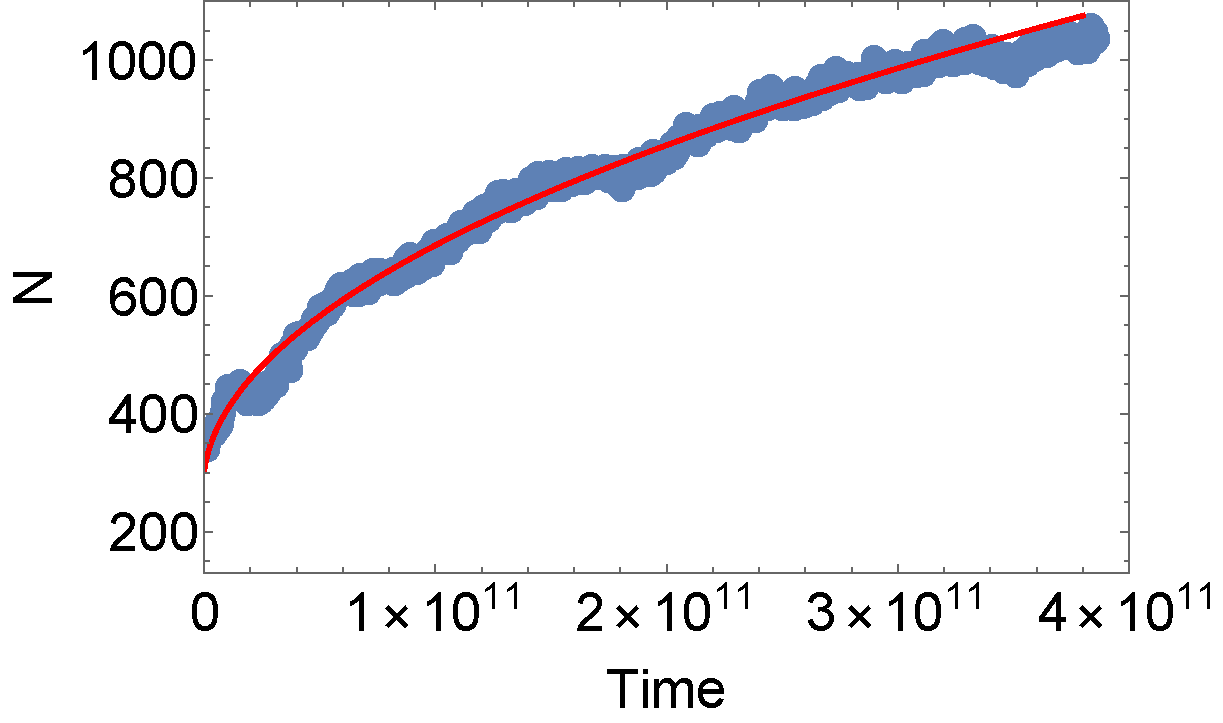
\includegraphics[scale=0.5]{longtrajectoryFig2.pdf}
\caption{$N$ vs. $t$. The growth rate here is for $\delta \mu = 0.18$ with $k_s=4$ and $k_\theta = 6$.} \label{fig:GrowthRate}
\end{figure}
\begin{figure}
\centering
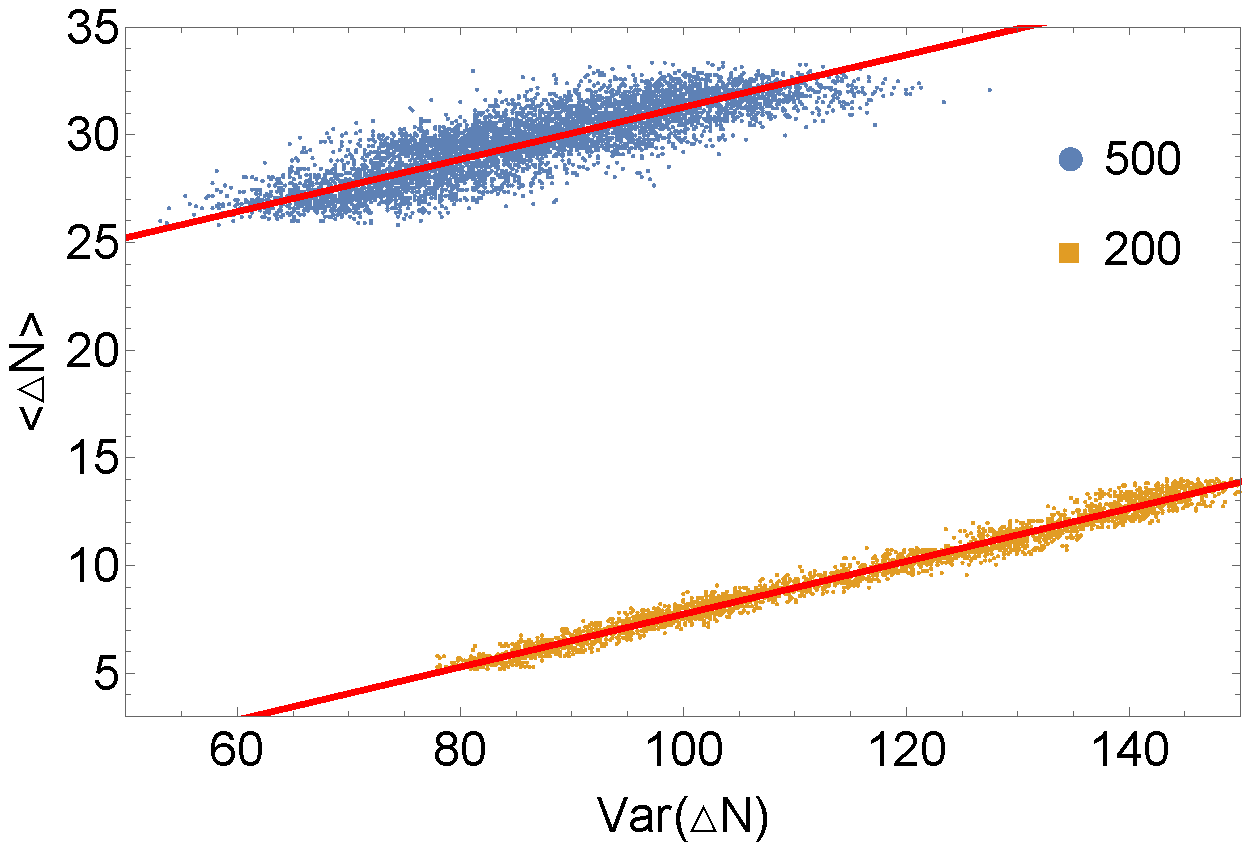
\includegraphics[scale=0.4]{deltaNvsVarFig3.pdf}
\caption{$\Delta N$ vs. $Var(\Delta N)$ for different $N_0$. The slope extracted here is approximately 0.09 making $\frac{v}{D}=0.18$. The data here is for $\delta\mu=0.18$, $k_s=4$ and $k_\theta = 6$.} \label{fig:growthvsvariance}
\end{figure}


%\section{Small n modes deviation}
%The smallest n modes show some deviation from the Helfrich description as shown in the Fig.~\ref{fig:fit} . The deviation seems to be an apparent increase in the surface tension. This effect might be because the number of the particle $N$ in this simulations is always changing. Thus this might make difficult for the longest wavelength move to relax. In this paper, we have reported the $\gamma$ extracted from the bigger n modes. 
%\begin{figure}[tbb]
%\centering
%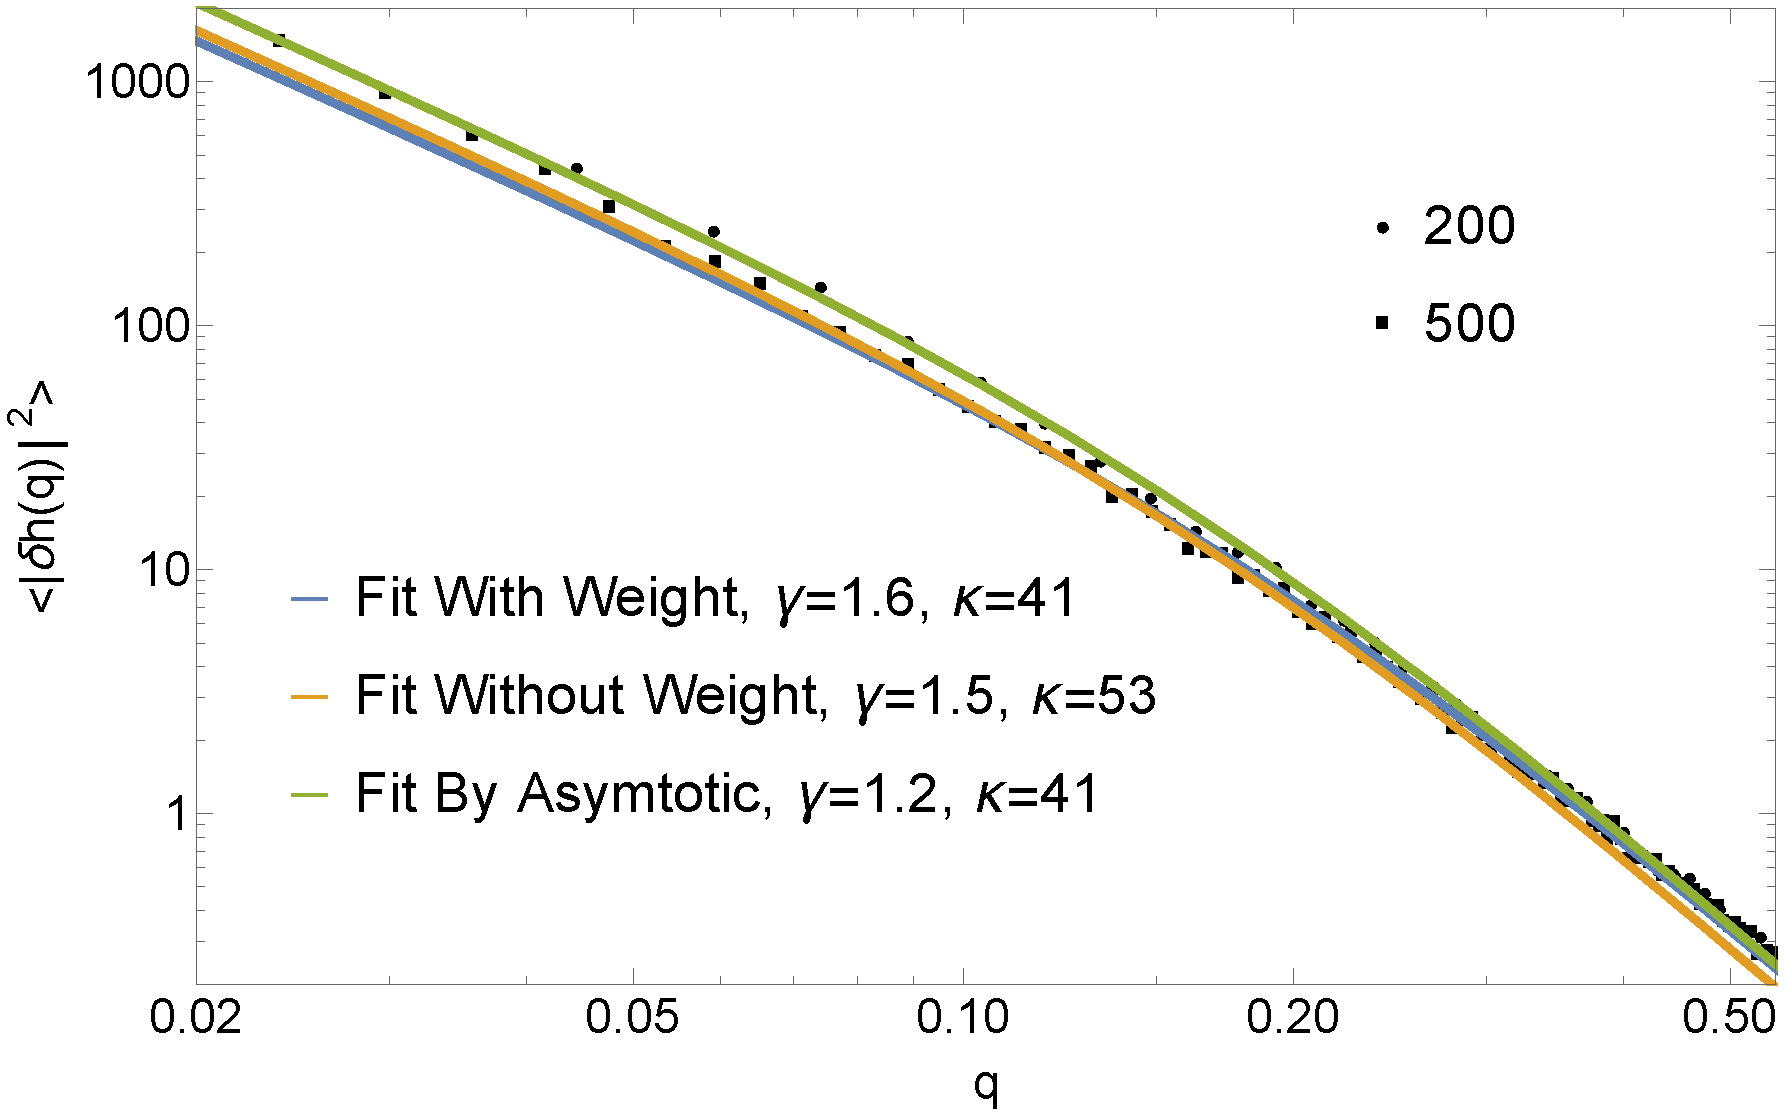
\includegraphics[scale=0.30]{fittingandsmallneffect.pdf}
%\caption{$\langle|\delta %h(q)|^2\rangle$ vs. $q$ for $\delta %\mu \approx 0$ with $k_s=4$ and %$k_\theta = 6$. For the smallest n %modes, both the 200 and 500 particles %spectrums converge to the $\gamma=1.2$ %while the rest of the n modes follow %$\gamma=1.6$ } \label{fig:fit}
%\end{figure}
%\section{Fitting Procedure}
%In order to extract $\gamma$ and $\kappa$ we need to fit $\langle|\delta h(q)|^2\rangle$ to $\frac{1}{\gamma q^2 +\kappa q^4}$. However, to fit the function correctly, we have to take into account that the variance of the spectrum is not constant. Specifically, the standard deviation of this spectrum is equal to its average. In order words, the errors in measuring in amplitude of the long wavelength modes will be significantly higher than the errors in measuring the amplitudes of the short wavelength ones. This is because each mode can be independently described with an exponential distribution. To fit the spectrum, we have to adjust the weight of the variances in the fitting procedure: $\rm{Weight(q)} = \frac{1}{\rm{Var(\langle|\delta h|\rangle ^2)}}$ so that we do not overfit the long wavelength region.

\section{Predicting effective elastic constants}

In the main text, we have used the bounds to predict the required $\delta \mu$ to attain certain effective tension, $\gamma_{\textrm{eff}}$. In a different way, we can use the bounds to predict how increasing $\delta \mu$ affect the surface tension. Fig~\ref{fig:epsilonpredict} shows how Eq. 7 and Eq. 8 in the main text, can be used to predict $\gamma_{\textrm{eff}}$. From the predicted $\gamma_{\textrm{eff}}$, we can construct an effective fluctuation of the interface when it is out of equilibrium. 
\begin{figure}[tbb]
\centering
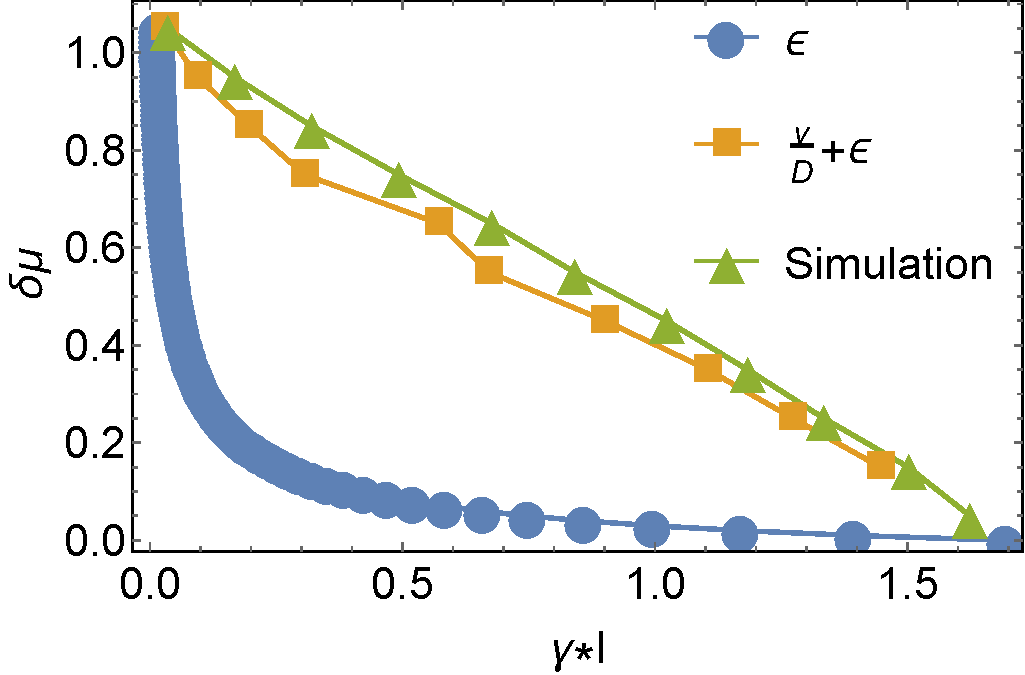
\includegraphics[scale=0.5]{predictepsilonv2Fig4.pdf}
\caption{$\delta\mu$ vs. $\gamma$. Instead of predicting the required $\delta\mu$, the blue curve (from Eq. 7) and the orange curve (from Eq. 8) can be used to predict the effective surface tension at certain $\delta \mu$. The data here is for $k_s=4$ and $k_\theta = 6$.} \label{fig:epsilonpredict}
\end{figure}
%P(l_{BE},l_{EC},l_{BC},\widehat{BEC},\widehat{ABE},\widehat{ECD},\widehat{ABC},\widehat{BCD})
% P(l_{BC},\widehat{ABC},\widehat{BCD})
%
%\begin{figure*}
%\centering
%  \subfloat[]{%
%   \includegraphics[scale=0.35]{estimationfordeltamu0d1ver2.pdf}}\hfill
% \subfloat[]{%
%    \includegraphics[scale=0.35]{estimationfordeltamu0d4ver2.pdf}}\\
%  \subfloat[]{
%   \includegraphics[scale=0.35]{estimationfordeltamu0d7ver2.pdf}}\hfill
%  \subfloat[]{%
%    \includegraphics[scale=0.35]{estimationfordeltamu1d0ver2.pdf}}\hfill
%\caption{Comparison of the Fourier Spectrums of the interface's fluctuation at different $\delta\mu$ from simulations and predicted by Eq. 8 in the main text. The data here is for $k_s=4$ and $k_\theta = 6$.} \label{fig:predictandsimulation}
%\end{figure*}


\bibliography{References02232018}
\end{document}